\documentclass{article}

\usepackage{multicol}
\usepackage{lipsum}
\usepackage{graphicx}
\graphicspath{{images/}}
\usepackage{blindtext}
\usepackage{subfiles} % Best loaded last in the preamble
\usepackage[dvipsnames]{xcolor}
\usepackage[T1]{fontenc}
\usepackage{setspace}
\usepackage{float}

\setlength{\columnsep}{1cm}

\usepackage{fullpage, tikz}
\usepackage{eso-pic}
\AddToShipoutPictureBG{%
	\begin{tikzpicture}[remember picture, overlay]
		\node[opacity=.4, inner sep=0pt]
		at(current page.center){
\includegraphics[width=8.5in, height=11in]{images/background}};
	\end{tikzpicture}%
}

\usepackage[margin={1.5cm,1.5cm}]{geometry}

\newcommand\BackgroundPic{%
	\put(0,0){%
		\parbox[b][\paperheight]{\paperwidth}{%
			\vfill
			\centering
			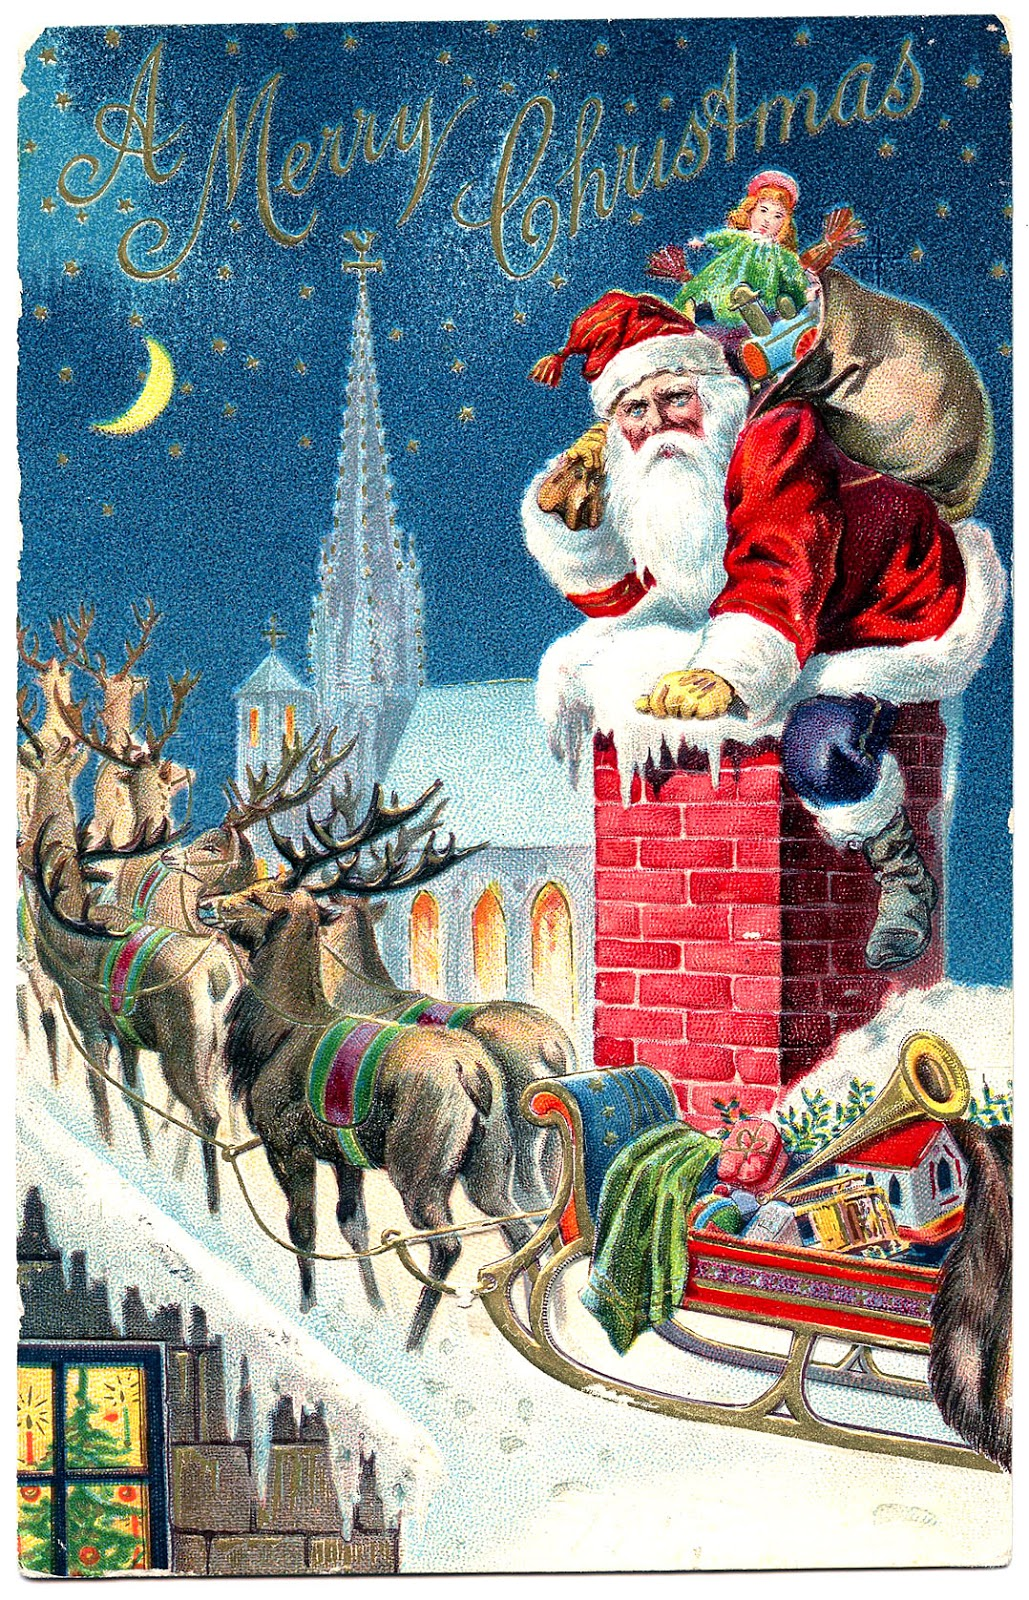
\includegraphics[width=\paperwidth,height=\paperheight]{images/cover.jpg}%
			\vfill
}}}

\title{\color{white}\textsc{\Huge Winter Solstice Sabotage }}
\date{ }


\setlength\fboxsep{8pt}

\begin{document}
	\AddToShipoutPicture*{\BackgroundPic}
	\maketitle
	\pagebreak
	\begin{multicols*}{2}
	\section{Introduction}
	
	\subsection*{Overview}
	The \emph{Winter Solstice Sabotage} one-off adventures is meant to be played with a group of 5 players at level 4. The adventure is meant to be completed in one session.
	
	It is a Christmas inspired story with familiar themes and characters. The plot of the story revolves around the character \emph{Klauss Atnas} (Santa Claus) whom has lost his powers to an evil gnome named \emph{Mister Frink}. The adventurers must help \emph{Klauss} find the evil gnome and defeat him to lift the curse and restore the blessing of the winter solstice.
	
	\subsection*{Adventure Hook}
	After a long year of adventures and treasure hunting, the adventurers find themselves returning home to celebrate the winter solstice when they are caught in a massive blizzard. They are forced to stop and find shelter, and happen to come across a tavern called the \emph{The Jolly Reindeer}. They enjoy a quiet meal with other guests lost in the storm when suddenly they hear a loud thump on which appears to come from the roof. Terrified, the hosts and other patrons try to convince the adventurers to go investigate what caused the loud noise on the roof.
	
	Upon investigating they find Klauss Atnas (Santa Claus) kneeling down below a large slay pulled by strange creatures with large antlers. Klauss is an other white bearded gnome wearing a Santa style robe and hat. Klauss appears to be attempting to fix the giant slay when he is startled by the adventurers. In a panic he attempts to activate his invisibility necklace but is unaware that the necklace's power has faded and is not concealing him. Once he realizes that the players can see and hear him, he explains who he is and how he brings blessings to each home in the world during the winter solstice festival. When he realizes that his powers have gone, he tries to recruit the adventurers to help him solve this mystery. The assumption here is the players will agree to this to move the story along, otherwise Klauss will simply kidnap them.
	
	Due to the emergency, Klauss uses an emergency magical device which transports him and all the players to what is suppose to be Northerland (north pole). Unfortunately the device malfunctions and they find themselves outside the Northerlands in a snowy plains in the middle of blizzards. Confused, it takes Klauss a moment to comprehend the malfunction and realize where they are located. He looks at his compass it is completely indicating the wrong direction. After some time he finally is able to determine his location and remembers an ancient cave used in the past for tracking winter solstice operations. 
	
	\section{The Adventure}
	\subsection*{\underline{1. The Abandoned Cavern}}
	
	Klauss leads the players to an abandoned cave which once acted as a base of operations for the winter solstice festival blessing. The entrance of the cave is dark and there appears to be a large locked metal door. Klauss tries to remember the password but can't remember exactly (get creative with password ideas). He finally gets the right password (two turtledoves and a partridge in a pear tree). The door opens and torches light to illuminate a large cavern. Klauss rushes to the other side of the cavern where a console with various controls is located.
	
	Klauss fails to notice a hidden \emph{Snow Owlbear} hidden in the snow around the cavern. Unless the players proceed carefully by using perception, investigation or stealth, the \emph{Snow Owlbear} surprises the adventurers (run the owlbear encounter). Klauss will join the fight although we is generally not a fighter, he mainly focuses on using his protective and defensive abilities to help the adventurers.
	
	Once the owlbear is defeated, it drops a lump of coal with a strange symbol on it. Klauss immediately recognizes it as \emph{Mr. Frink}'s calling card. To his dismay, it appears \emph{Mr. Frink} has somehow infiltrated the Northerland village and has corrupted it's magical powers. Klauss asks the players to travel to Northerland village and attempt to find and apprehend Mr. Frink before the winter solstice festival is over. He hands the players a working compass which will lead them to the Northerland village. In addition, he gives them the defective device which contains the corrupted device and asks the adventurers if they can get help from the other gnomes to discover why it's been corrupted.
	
	\colorbox{GreenYellow}{\begin{minipage}{0.4\textwidth}
		Players who investigate the corrupted device learn that it's compass actually points in the exact opposite direction as the functioning device. In fact, the adventurers should learn later that Mr. Frink's presence repels the compass' needle. The players can use this to determine which of the gnomes is in fact \emph{Frink}. 			
	\end{minipage}}
	\break
	
	Klauss must continue his blessing delivery if he is to complete it before the end of the winter solstice. He manages to tap enough magical energy from the console to power his slay and reindeer to continue his journey. Before he leaves them, he gives them custody of Durolph the red nosed reindeer to ride to the Northerland village. Durolph grows large enough to accommodate all the adventurers to ride it. He also urges the adventurers to hurry because Mr. Frink's power grows every passing moment. 
	
	\subsubsection*{\underline{2. Northerland Village}}

	The adventurers travel on Durolph's back through the snow planes and blizzard towards Northerland village. After about an hour of travel, they finally arrive at a lone small log cabin covered in snow. The gnome clerk at the desk doesn't appear to be paying attention to the players. Once the clerk realizes that the adventurers are not the regular visitors he is accustomed to, he is surprised and nervous. The players will have to persuade him the let them into the village, with advantage if they show him Klauss' devices. The clerk doesn't know much about Mr. Frink and finds the idea of him infiltrating Northerland village laughable.
	
	Once persuaded, the clerk let's the players through a back door which opens to another world. Northerland village is a bustling town full of gnomes who are especially busy during the winter solstice celebration. The village contains many homes and factories where gnomes are working on building statues and idols used in the blessings. The village is protected by a giant magical bubble shield. There are thousands of gnomes running around, so finding the impostor Mr. Frink will be like trying to find a needle in a haystack. Most of the gnomes are so busy they just completely ignore the players.
	
	At this point, you should start some sort of timer or keep track of the players actions to determine how much time has passed. Mr. Frink starts with a power level of 3 (increase to 4 or 5 to increase the difficulty). You can periodically increase his power at your discretion if the players are taking to long or are failing to progress towards finding him. Keep track of his power level as it will determine how many clones and how strong Mr. Frink will be.
	
	The easiest way to find Mr. Frink is to use the corrupted compass. The closer the compass is to Frink, the more the needle will vibrate. The needle will always point away from him, so it can be used as a guide. The players might be savvy enough to determine this without extra clues, but if not, they will need to investigate around town to find more clues.
	
	\subsubsection*{\underline{3. Northerland Administration Office}}
	
	In the center of the town is a the main administration building where players can find extra clues to help in their investigation in finding Frink. The head administrator gnome named \emph{Frosty} can provide some information for the players. He is more inclined to take the Mr. Frink threat seriously. He is aware of the basic history and legends surrounding him but will need to check the archives.
	
	If the players choose to try to find clues in the archives, add a level of power to Mr. Frink. In the archives, the players can use any intelligence skill they desire to search the archive records. Based on the skill type and roll, players can discover clues about Mr. Frink.
	
	\underline{\textbf{Arcana Roll Table}}
	\begin{description}
		\item[1-4] Failure, add +1 power level to Mr. Frink.
		\item[5-8] No clue
		\item[9-12] Mr. Frink is a master of disguise and it is said that he can even magically replicate himself.
		\item[13-15] Destroying his clones will reveal his true identity.
		\item[16-18] Mr Frink is vulnerable to fire.
		\item[>19] Mr. Frink's clones can be destroyed by solving riddles or by attacking the real him. Hurting a clone or failing to answer the riddle will freeze the target. 
	\end{description}

	\underline{\textbf{History Roll Table}}
	\begin{description}
		\item[1-4] Failure, add +1 power level to Mr. Frink.
		\item[5-8] No clue
		\item[9-12] Mr. Frink is a master of disguise and it is said that he can even magically replicate himself.
		\item[13-15] Destroying his clones will reveal his true identity.
		\item[16-18] Mr Fink is vulnerable to fire.
		\item[>19] Mr. Fink's clones can be destroyed by solving riddles or by attacking the real him. Hurting a clone or failing to answer the riddle will freeze the target. 
	\end{description}
	

	\subsubsection*{\underline{2. Main Telescope Room}}
	The main telescope room is in complete disarray. What was once a technological marvel has now been damaged beyond repair left to rust away. The main telescope is a very large lens that appears to be pointing out into the night sky, but isn't functional. The controls to move it have been broken and rendered unusable. Debris litters the floor showing signs of a fight occurring in this room. The players may investigate the room but all that can be found are various documents and old reports which appear to have faded with time. There are three additional doors in the main room. The western door leads to \emph{area 3} which is the main laboratory. The eastern door leads to Frunsmag's office \emph{area 4}. The northern door (\emph{area 5}) has been barricaded and leads down to the ancient telescope.
	
	\subsubsection*{\underline{3. Laboratory}}
	The laboratory is not in any much better state than any of the other rooms. It contains many spilled over or abandoned experiments. The floors are covered with sharp broken glass from broken tubes and various other glass labware. Any player investigating the room require a DC 10 acrobatic check or take 1d6 slashing damage upon falling. The only object of value in this room is a \textbf{Potion of Time Rejuvenation} but the players will need a DC 15 investigation check to find it. Unless they have found the similar vial in Frunsmag's office, identifying the potion requires a DC 15 arcana or medicine check. 
	
	\subsubsection*{\underline{4. Frunsmag's Office}}
	Frunsmag's used this office to try to find an escape from the observatory when he was still alive. The walls are covered with writings of what appears to be someone completely going mad. Most of the writing is along the lines of "NO TIME", "DEATH IS WELCOMED HERE", "ESCAPE". In the corner of the room is a bed containing the remains of Frunsmag. Investigating the body reveals it appears he died of old age, over a hundred years ago.
	
	The room contains a desk with scattered papers and Frunsmag's journal. The journal contains a log of Frunsmag's captivity in the observatory. The first few entries are dated a month back, but later entries have the date marked as unknown (apparently Frunsmag had lost track of time). The gist of the entries include Frunsmag's day to day life, various attempts to escape. One entry mentions his colleagues going down to the ancient telescope to try to find a way out and them being killed by a strange creature. The final entry in the journal reads:
	
	
	
	\subsubsection*{\underline{5. Barricaded Door}}
	The door has been barricaded and requires a DC 15 strength check to clear the debris blocking the door. A failure of on this check causes debris to fall on whomever is around for 2d6 of bludgeoning damage. The second attempt requires a DC 10 strength check and deals 1d6 on failure, and the debris is cleared completely. The door opens to a long staircase that leads to the ancient telescope, deep underground inside the mountain.
	
	\begin{figure*}
	\centering
	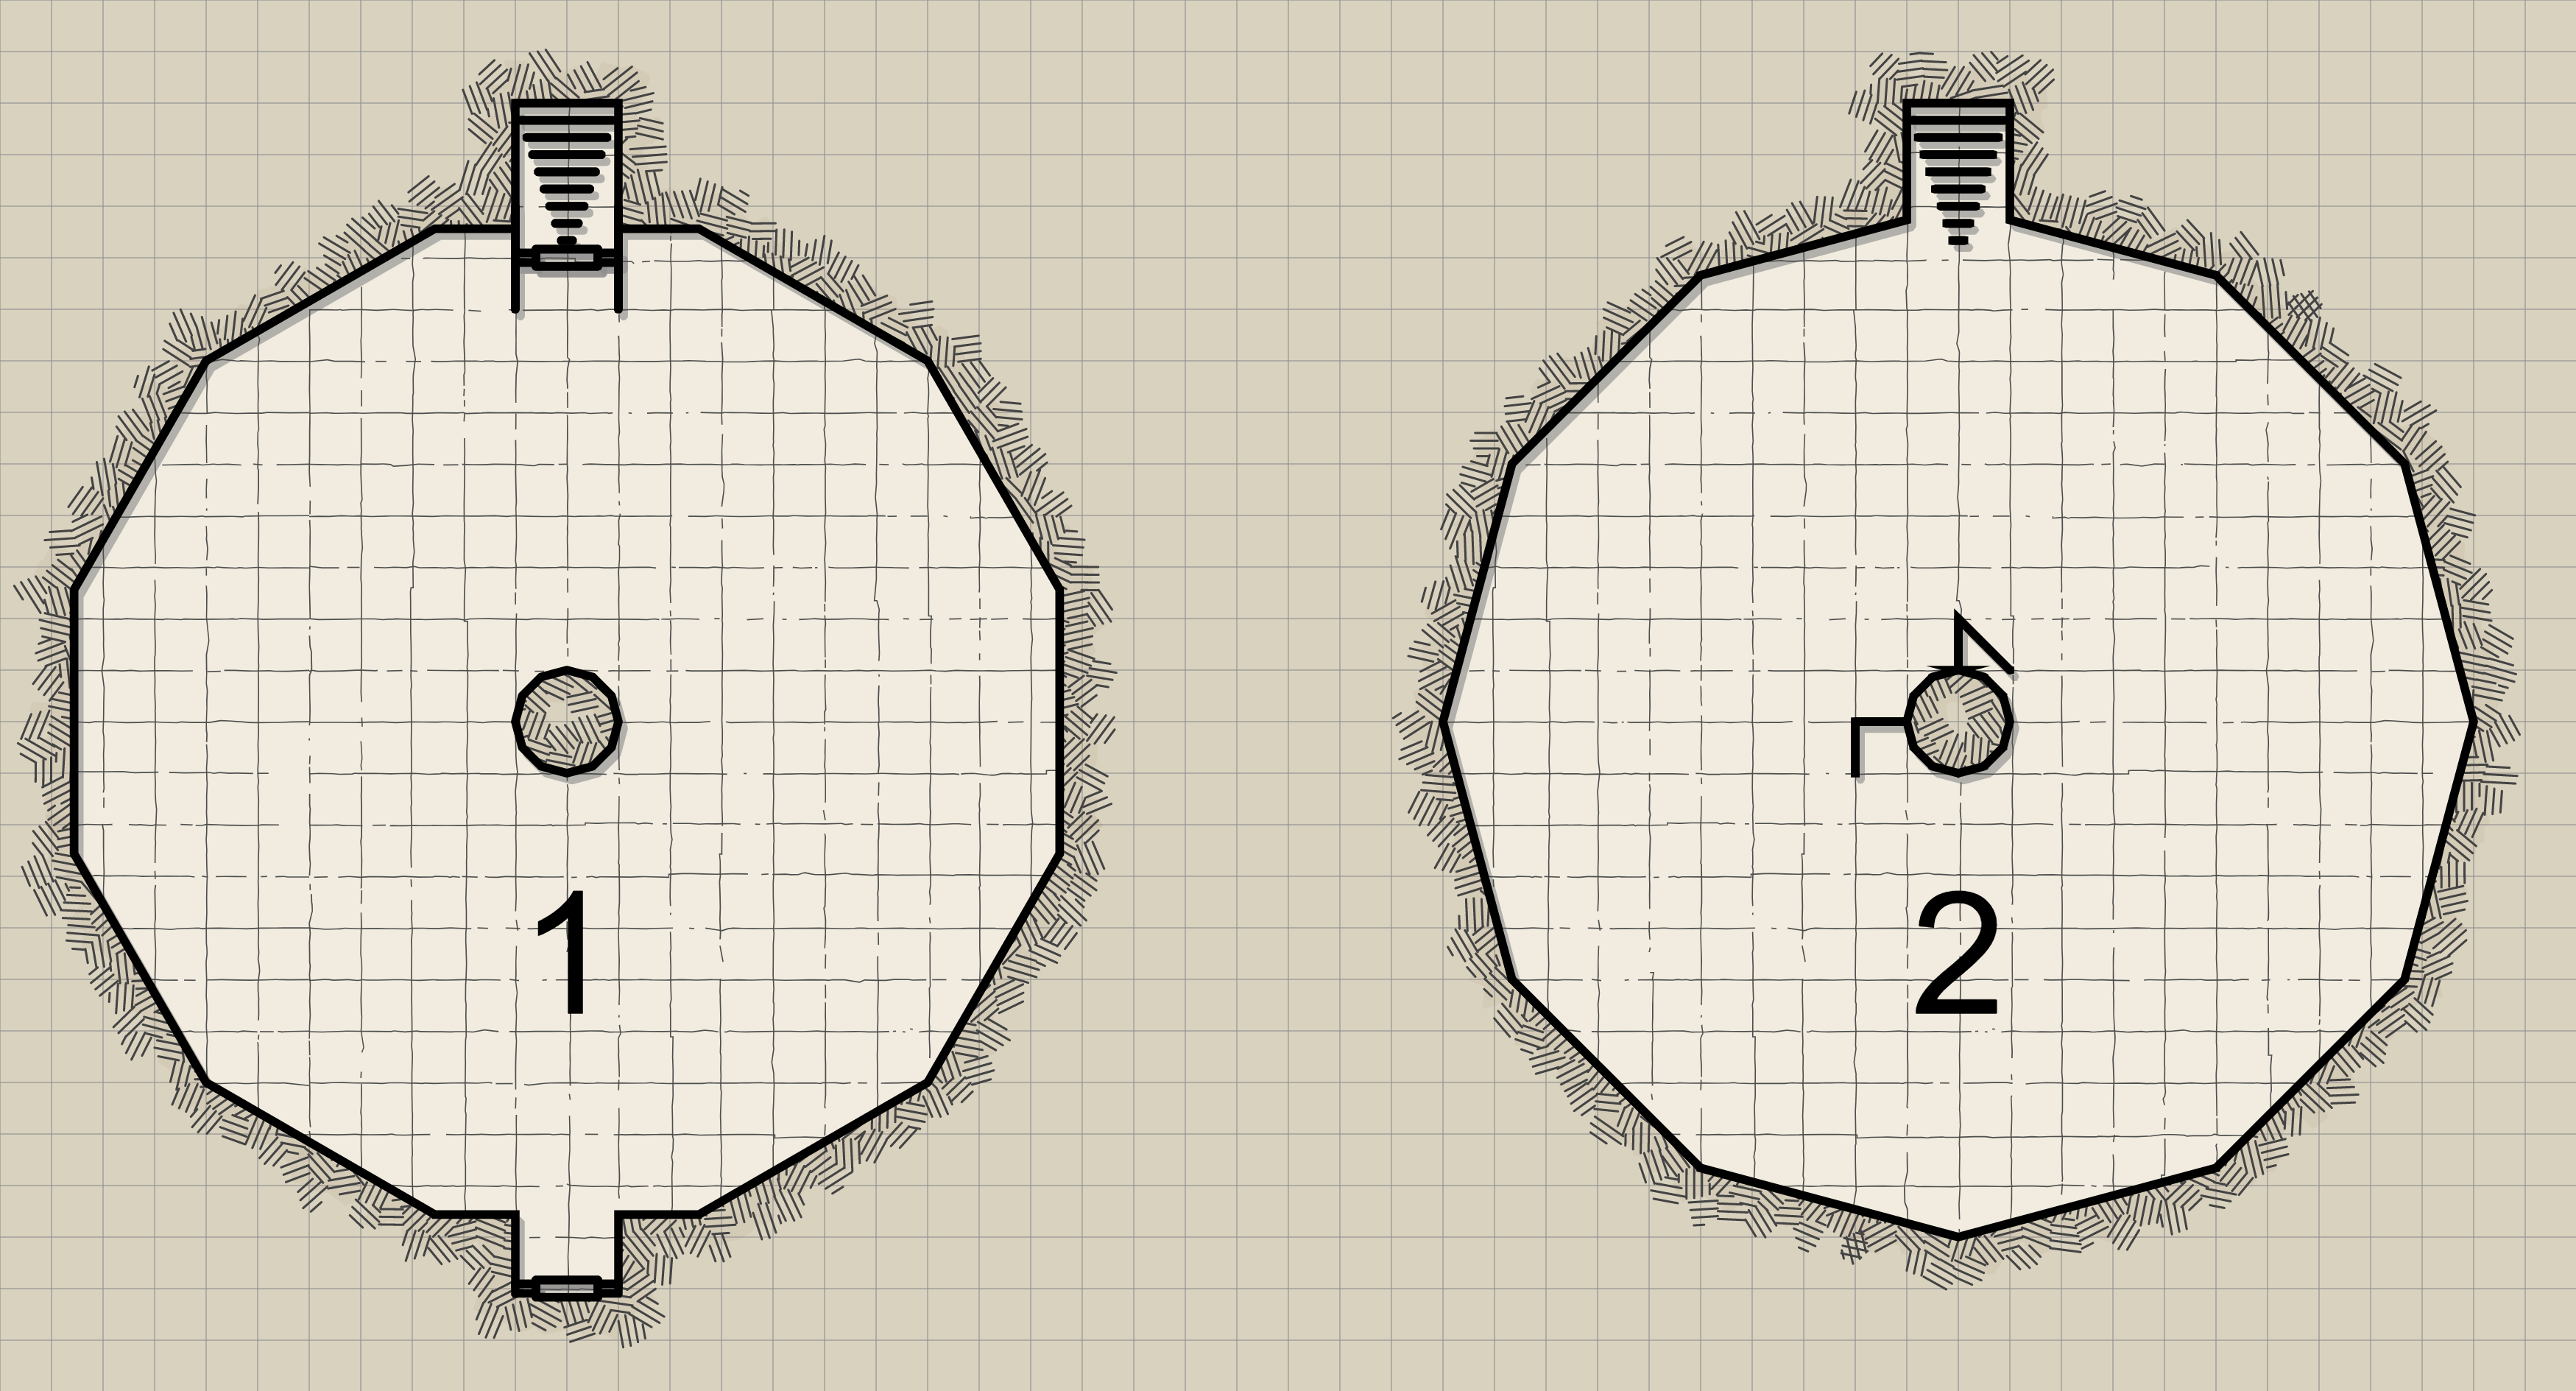
\includegraphics[width=0.8\textwidth]{images/ancient_telescope}
	\caption{The Valboro Observatory Top Level}
	\end{figure*}
	\section{The Ancient Telescope}
	Once the debris has been cleared, the door in \emph{area 5} opens to a long staircase leading deep into the mountain. At the bottom of the staircase, a mile long straight dimly lit corridor leads to a closed door. The door opens to \emph{area 1} in the ancient library room. Once the players have entered into the library, they are now trapped in this room. Trying to escape through the door takes them into a copy of the library room, similar to the phenomenon occurring at the observatory's entrance.
	
	\subsubsection*{\underline{1. Ancient Library}}
	The ancient library is a large circular room which contains wall to wall bookshelves full of ancient and modern science, history, and mythology books. However, something unusual is happening in this room, gravity appears to be reversed. The room is actually upside down, the players are in fact standing on the ceiling. Knock over books cover the floor above the players heads. If they attempt to touch any of the objects, the objects react and fall down to the ceiling.
	
	In the center of the room is located the ancient telescope. The ancient telescope is essentially an 10 foot diameter shaft which was drilled straight through the mountain with lenses positioned at intervals within the shaft to provide maximal magnification. However, since the room is upside down, the shaft appears to be point down into the ceiling. On the other side (above the player's heads) is the other end of the telescope. From this room, the players can only see some sort of reflective surface at the bottom, which is actually the mirror found in \emph{area 2}. The telescope appears to be pointed directly at some sort of constellation:
	
	\begin{center}
		
\includegraphics[width = 0.3\textwidth]{images/constellation}
		
		\emph{Hourglass Constellation}
	\end{center}

	The hourglass constellation is the root cause of what is happening in the observatory. Every few centuries, when the constellation aligns with the ancient telescope, it creates a time rift. The \emph{Time Harvester} uses this event as an opportunity to siphon time from this dimension. In order for the party to close the rift, the players will need to align the mirror in \emph{area 2} and jump through the shaft to transport to the harvester's universe.
	
	To the north of the room is a ladder leading down to \emph{area 2}.
	
	\subsubsection*{\underline{2. Constellation Chamber}}
	The constellation room is a circular dome-shaped room. The walls are arrayed with hundreds of different symbols which can be discovered to be various constellation formations upon a successful DC 10 arcana or history check. In the middle of the room is a mirror on a pedestal which is aligned directly with the telescope above it, and projects the image from the telescope onto the wall. The pedestal holding the mirror has two main levers which enables the mirror angle to be swiveled around so it can project  the image anywhere in the room.
	
	When the players first arrive in the room, the mirror is projecting the hourglass constellation onto a random spot on the wall. When the players attempt to approach the mirror, the \textbf{time guardian} and  \textbf{two temporal elementals} climb out from the mirror. Once the guardian is defeated, it vanishes into a hazy ripply cloud covering the entire floor. Every round a creature stands in the cloud, they must perform the DC 12 constitution saving throw or be affected by \emph{time's grasp} (see the \textbf{time guardian} stats for details, but no necrotic damage dealt).
	
	In order to breach the time rift, the players must align the mirror's projection with the correct constellation. Finding the correct constellation will require a group effort of investigation checks. Before beginning the rounds of investigation, each player will perform either an arcana or a history check to determine their ability to identify constellation symbols. The symbols are aligned in a logical and chronological pattern, therefore players who succeed a DC 15 arcana or history check will have advantage on their investigation rolls. Once investigation starts (use the same initiative order from the previous combat), each player rolls for investigation. Finding the correct symbol will require a successful DC 25 investigation check (decreases by 5 every round). Remember to perform the checks for the time's grasp cloud.
	 
	The correct symbol is the hourglass constellation. Once found, at least one character must swivel the mirror to project the image onto the correct symbol. Once aligned, the time cloud dissipates, a loud ringing sound can be heard, and a bright light emerges from the symbol on the wall flowing into the mirror and upward through the telescope. The time rift is now successfully opened.
	
	\section{The Time Harvester's Lair}
	With the rift now open, the players should return back up the library. The library has now been restored back to it's correct upright position. The light coming from the mirror below can be seen rushing up through the telescope. Characters that step onto the light are transported directly to the Time Harvester's lair.
	
	The lair is a brightly lit circular dome shaped room similar to the constellation chamber. In the middle of the room is a giant floating golden hourglass, where the sand looks like bright energy specks and appears to be flowing in both directions inside the glass. Behind the hourglass, the \textbf{Time Harvester} can be seen performing some sort of ritual at an alter. He notices the intruders and stops the ritual. The players may choose to interact with him, but regardless, the time harvester is only interested in harvesting energy through time.
	
	There are two ways to defeat him, either by killing him or by destroying the golden hourglass. The hourglass has an AC of 20, and must be hit three (or more or less times if the difficulty needs to be adjusted) in order for it to be destroyed. Once defeated, the players are returned back to the observatory in the ancient library. 
	
	\section{Conclusion}
	Once returned back to the observatory, the players are free to leave and return back to Aleytheas for their reward. When they arrive in town, they find things have changed tremendously. The players return to the Winemakers Guild, but none of the administrators know anything about them or their quest. Upon discussions, the players realize the reason for this behavior. It seems time stood still in the observatory, but time continued on normally on the outside. Roll a d10 to determine how many centuries have passed since the players were sent on the quest. Once the administrators and historians researched the historical records, the heroes are given their promised reward of 10,000 gp.
	\vfill

	\pagebreak
	\section{Treasures}

\pagebreak
	
\section{Monsters}

\subsubsection*{Abruhani Pirates}

\subsubsection*{Child of Abruhan Cultist}

\end{multicols*}
	
\end{document}
